\documentclass[a4paper]{article}

\usepackage[utf8]{inputenc}
\usepackage[english]{babel}
\usepackage{hyperref}
\usepackage{graphicx}
\usepackage{amsmath,amssymb,amsthm}
\usepackage{siunitx}
\usepackage{xcolor}
\usepackage{multicol}
\usepackage{caption}
\usepackage{appendix}
\usepackage{pdfpages}
\usepackage{fixltx2e}
\usepackage[version=4]{mhchem}
\usepackage{url}
\usepackage{subcaption}

\date{\today}
\author{Thomas Brzeski \and  Victor Dejans}
\title{Kinematic and Dynamic Analysis of a Linkage\\ Walschaerts Valve Gear}


\begin{document}

\maketitle

\section*{Introduction}

In the context of the subject \textit{Beweging en trillingen (H01N0A)} this report treats the analysis of the linkage in a Walschaerts valve gear (as seen in figure~\ref{fig:basistekening}), a system that is used in steam locomotives.

In a first section we define all links and joints with their geometric properties in the way we used them for the assignment. We also make the motion analysis of the linkage.

Second is the kinematic analysis which finds the positions, velocities and accelerations of each bar.

The final section reports upon the inverse dynamic analysis which finds the forces and torques on the linkages' joints when a driving torque is applied to the train's wheel.



\begin{figure}[h]
	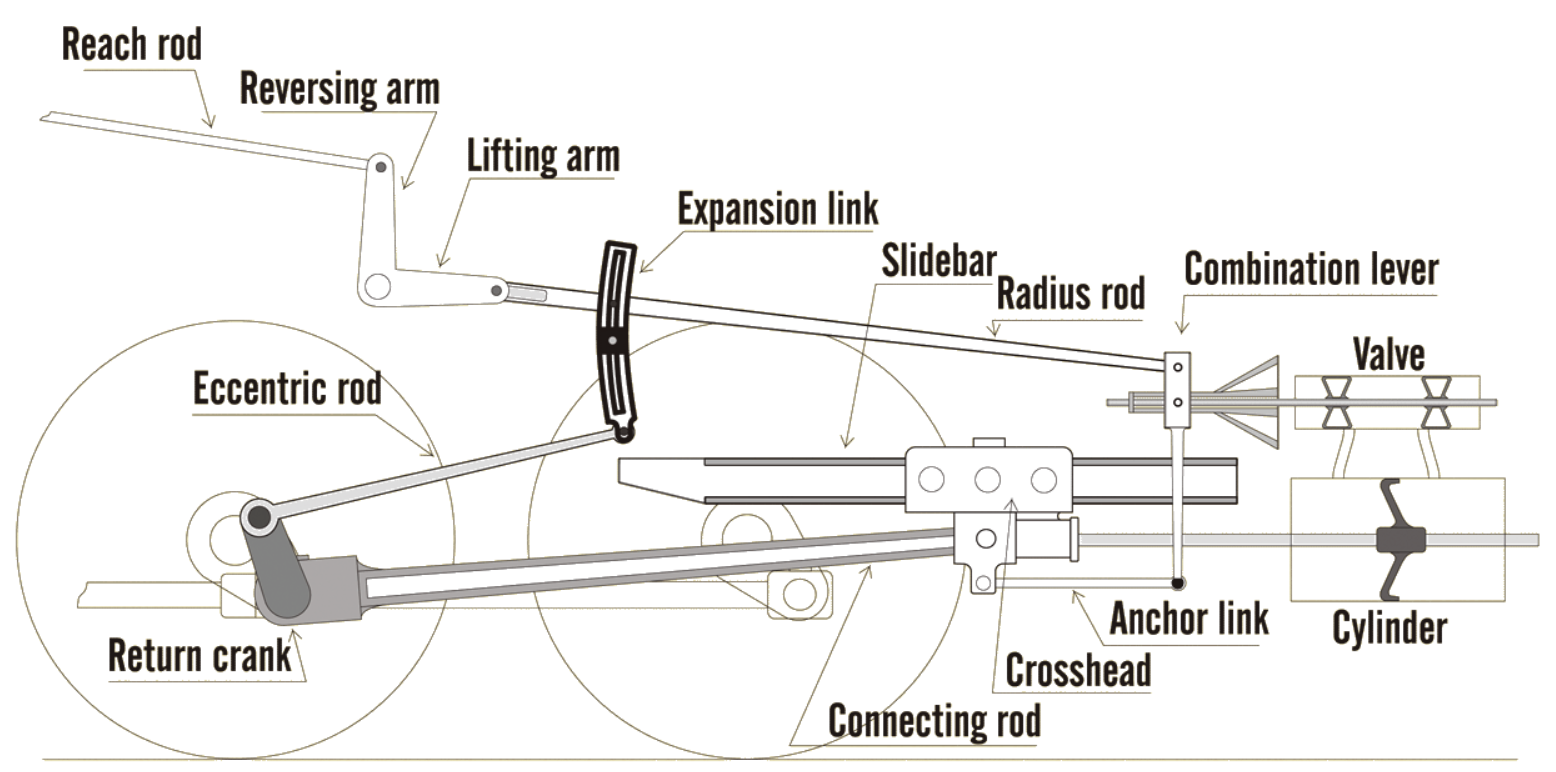
\includegraphics[width=0.9\textwidth]{wvgverslag.png}
	\centering
	\caption{Example of a Walschaerts valve gear. \cite{ove06}}
	\label{fig:basistekening}
\end{figure}

\newpage
\tableofcontents

\section{Definition of the mechanism}

Walschaerts valve gear is a linkage that was used in steam locomotives. It connects the steam pistons and the train's wheels in a way that also regulates the steam flow.

Although in real life the pistons are the driving bodies and the wheels is the driven bodies, the assistants recommended us to analyse the mechanism in the opposite way. In this assignment, the driving torque is thus applied to the wheel instead of the pistons.

\subsection{Schematic of the mechanism and definition of the parameters}

As shown in figure~\ref{fig:schematic}, the linkage has 12 bodies.

\begin{itemize}
	\item Body \textbf{(1)} is the train. This is the ground to which other bodies are fixed.
	\item Body \textbf{(2)} is the wheel of the train. Its rotation point (A) is fixed in the origin of the xy-plane. The ends of bars (3) and (12) are eccentrically attached to the wheel with hinges (B) and (C) respectively.
	\item Bodies \textbf{(3)}, \textbf{(4)}, \textbf{(7)}, \textbf{(8)}, \textbf{(10)} and \textbf{(12)} are straight bars with lengths as specified in table \ref{tab:dims}.
	\item Body \textbf{(5)} is massless and is used to make a special joint between bar (4) and bar (7). It is attached to bar (4) with a prismatic joint (I) and to bar (7) with a hinge (H).
	\item Bar \textbf{(6)} is a kinked bar which consists of two parts of 95~\si{cm} long that are fixed to each other in an angle of 90~\si{degrees}. The two ends of this L-shaped bar are fixed to the ground (1) and to bar (7) with hinges.
	\item Bodies \textbf{(9)} and \textbf{(11)} are the pistons of the valve gear. Both pistons are fixed to the ground (1) with prismatic joints that only allow movement in the x-direction. Their dimensions are shown in figure~\ref{fig:pistons}.
\end{itemize}

All bodies in this linkage are made of steel which has a density \(\rho_{steel} = 7800~\si{kg/m^3}\) \cite{steel1}.


\begin{figure}[h]
	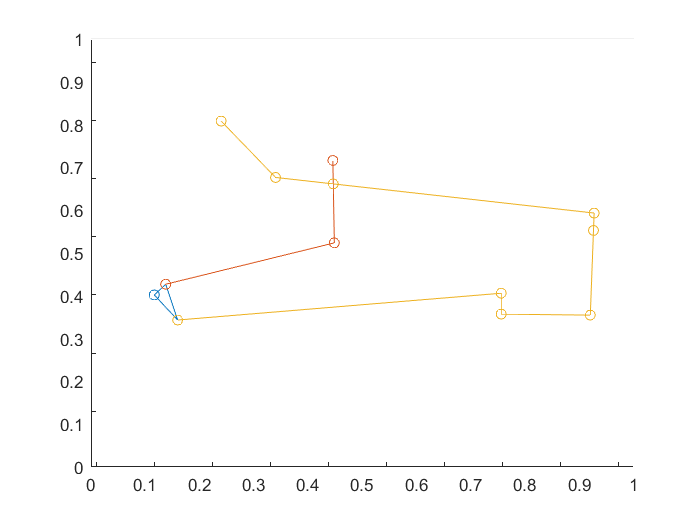
\includegraphics[width=\textwidth]{schematic.png}
	\centering
	\caption{Schematic representation of the studied linkage. The numbers indicate the 12 bodies. The letters indicate the 16 joints.}
	\label{fig:schematic}
\end{figure}


\begin{table}[h] 
	\centering
	\begin{tabular}{lc}
		\hline
		Bar & Length \((\si{cm})\) \\
		\hline
		2 between A and C & 27 \\
		2 between A and B & 59 \\
		3 between C and D & 299 \\
		4 between D and F & 142 \\
		6 between E and G (in a straight line) & 135 \\
		7 between G and H & 100 \\
		7 between H and J & 452 \\
		8 between J and K & 30 \\
		8 between K and M & 146 \\
		10 between O and M & 158 \\
		12 between B and N & 559 \\
		\hline
	\end{tabular}
	\caption{Dimensions of the bars and the wheel. Bars' numbers and joints' letters as indicated in figure~\ref{fig:schematic}.}
	\label{tab:dims}
\end{table}


\begin{figure}
	\centering
	
	\begin{subfigure}{.5\textwidth}
		\centering
		\caption{Piston (9)}
		\label{fig:piston9}
		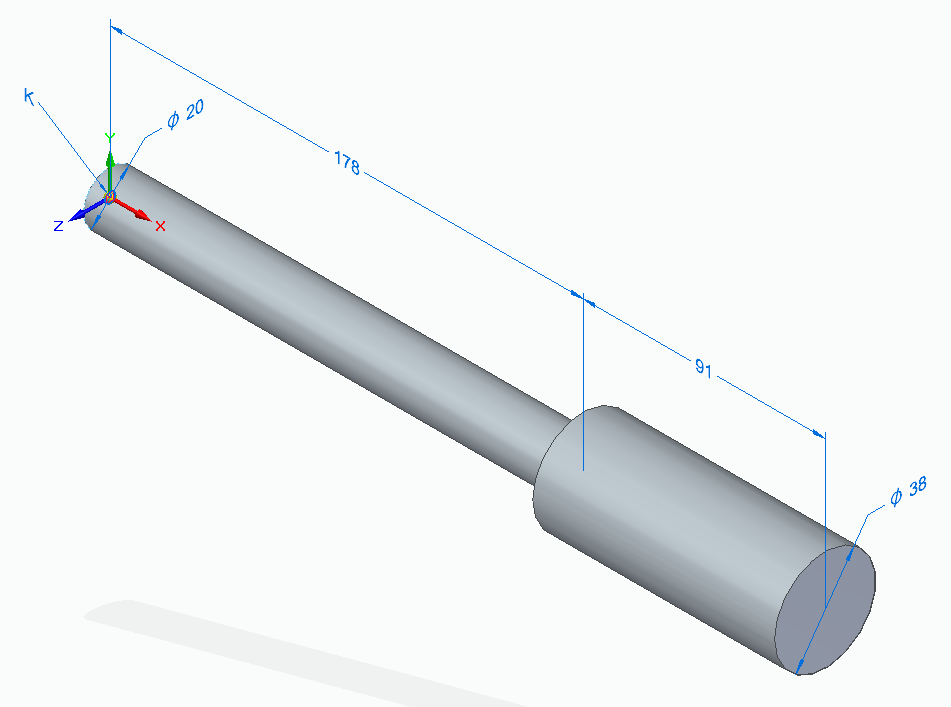
\includegraphics[width=.4\textwidth]{piston9.png}
	\end{subfigure}

	\begin{subfigure}{.5\textwidth}
		\centering
		\caption{Piston (11)}
		\label{fig:piston11}
		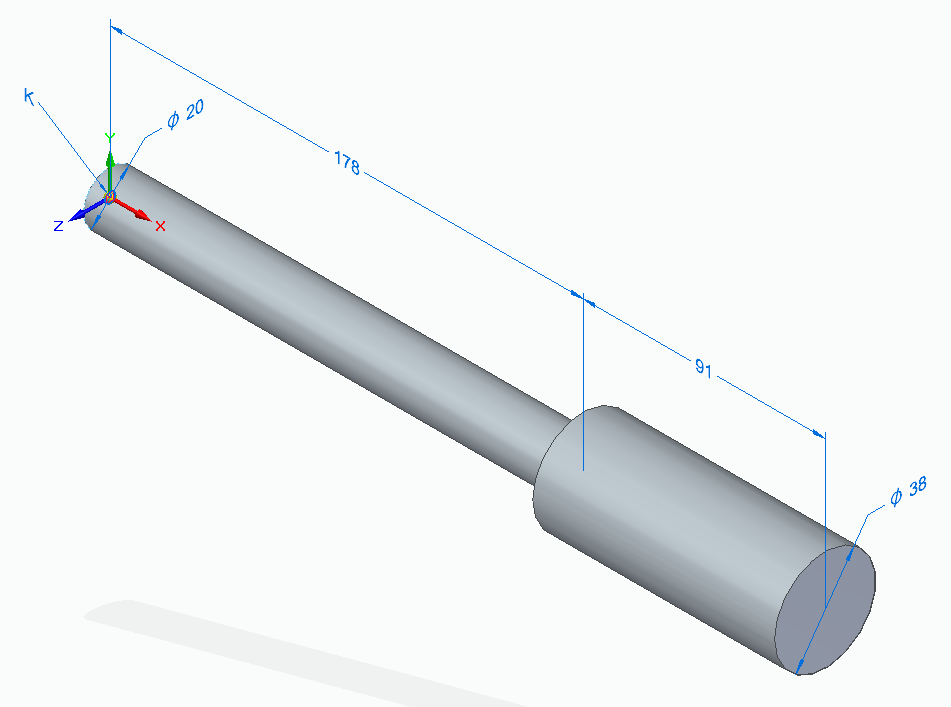
\includegraphics[width=.4\textwidth]{piston9.png}
	\end{subfigure}

	\caption{Pistons (9) and (11) with their dimensions and attachments to other bodies.}
	\label{fig:pistons}
	
%	https://tex.stackexchange.com/questions/37581/latex-figures-side-by-side
\end{figure}




\subsection{Motion analysis}

The Walschaerts valve gear is a 12 bar linkage system with 16 joints. This makes the mobility \(M=3*(12-1)-16*2=1\).






\section{Kinematic analysis}

\subsection{Loop closure equations}

\subsection{Position analysis}

\subsection{Velocity analysis}

\subsection{Acceleration analysis}

\subsection{Checking of results}

\section{Dynamic analysis}

\subsection{Inverse dynamic analysis without gravity}

\subsection{Inverse dynamic analysis with gravity}

\subsection{Checking of results}

\bibliographystyle{plain}
\bibliography{walschaerts}


\end{document}